\addchap{Anhang}
\begin{appendices}
	
	\begin{figure}[h]
		\centering
		\caption{Paketdiagramm der vorliegenden Softwarelösung}
		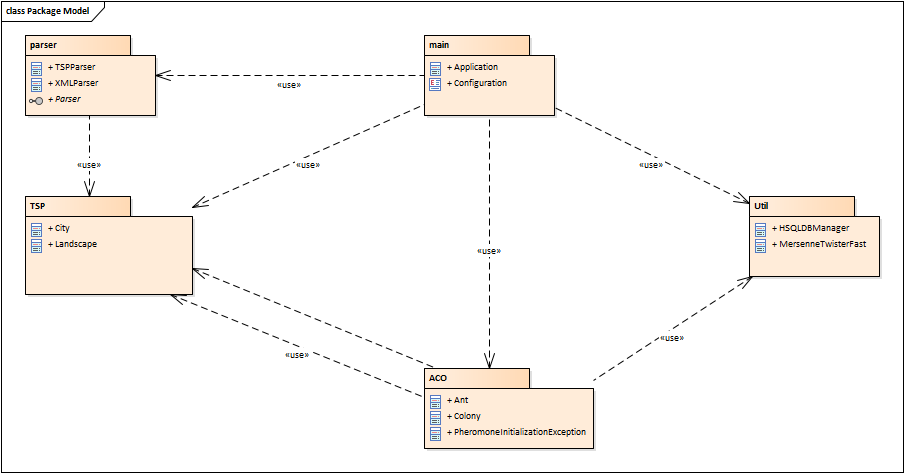
\includegraphics[width=\linewidth]{../../../01_uml/packageModel.png}
		\label{packageDiagram}
	\end{figure}

	\begin{figure}[h]
		\centering
		\caption{ER-Diagramm der vorliegenden Softwarelösung}
		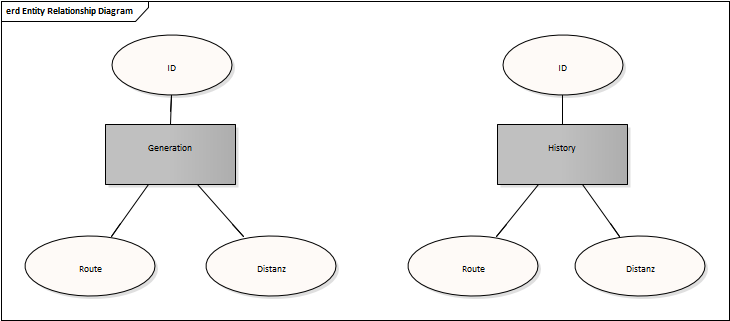
\includegraphics[width=\linewidth]{../../../01_uml/erDiagram.png}
		\label{erDiagram}
	\end{figure}

	\begin{figure}[h]
		\centering
		\caption{Testfälle der Klasse $Ant$, Seite 1}
		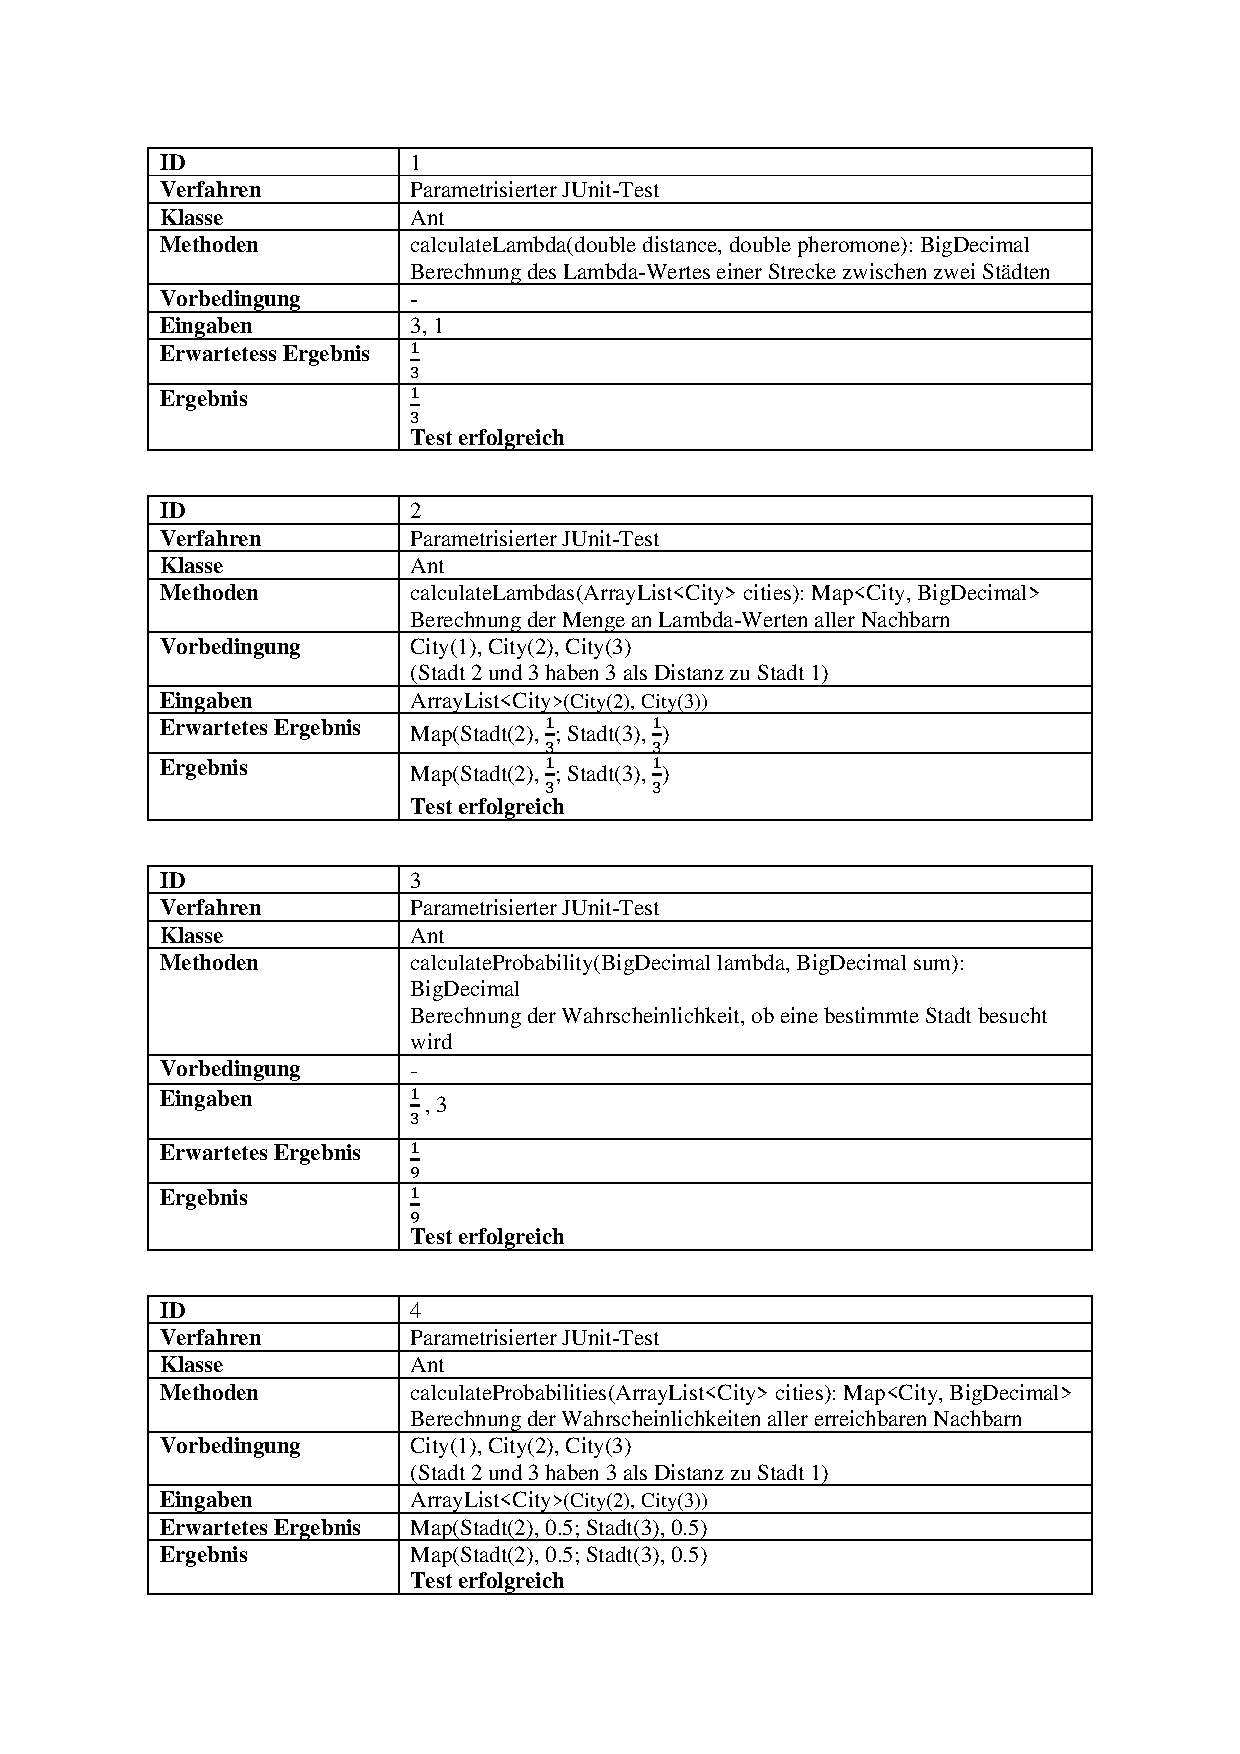
\includegraphics[width=\linewidth]{images/Testfaelle_Ant_Seite_1.pdf}
		\label{testAnt1}
	\end{figure}
	\begin{figure}[h]
		\centering
		\caption{Testfälle der Klasse $Ant$, Seite 2}
		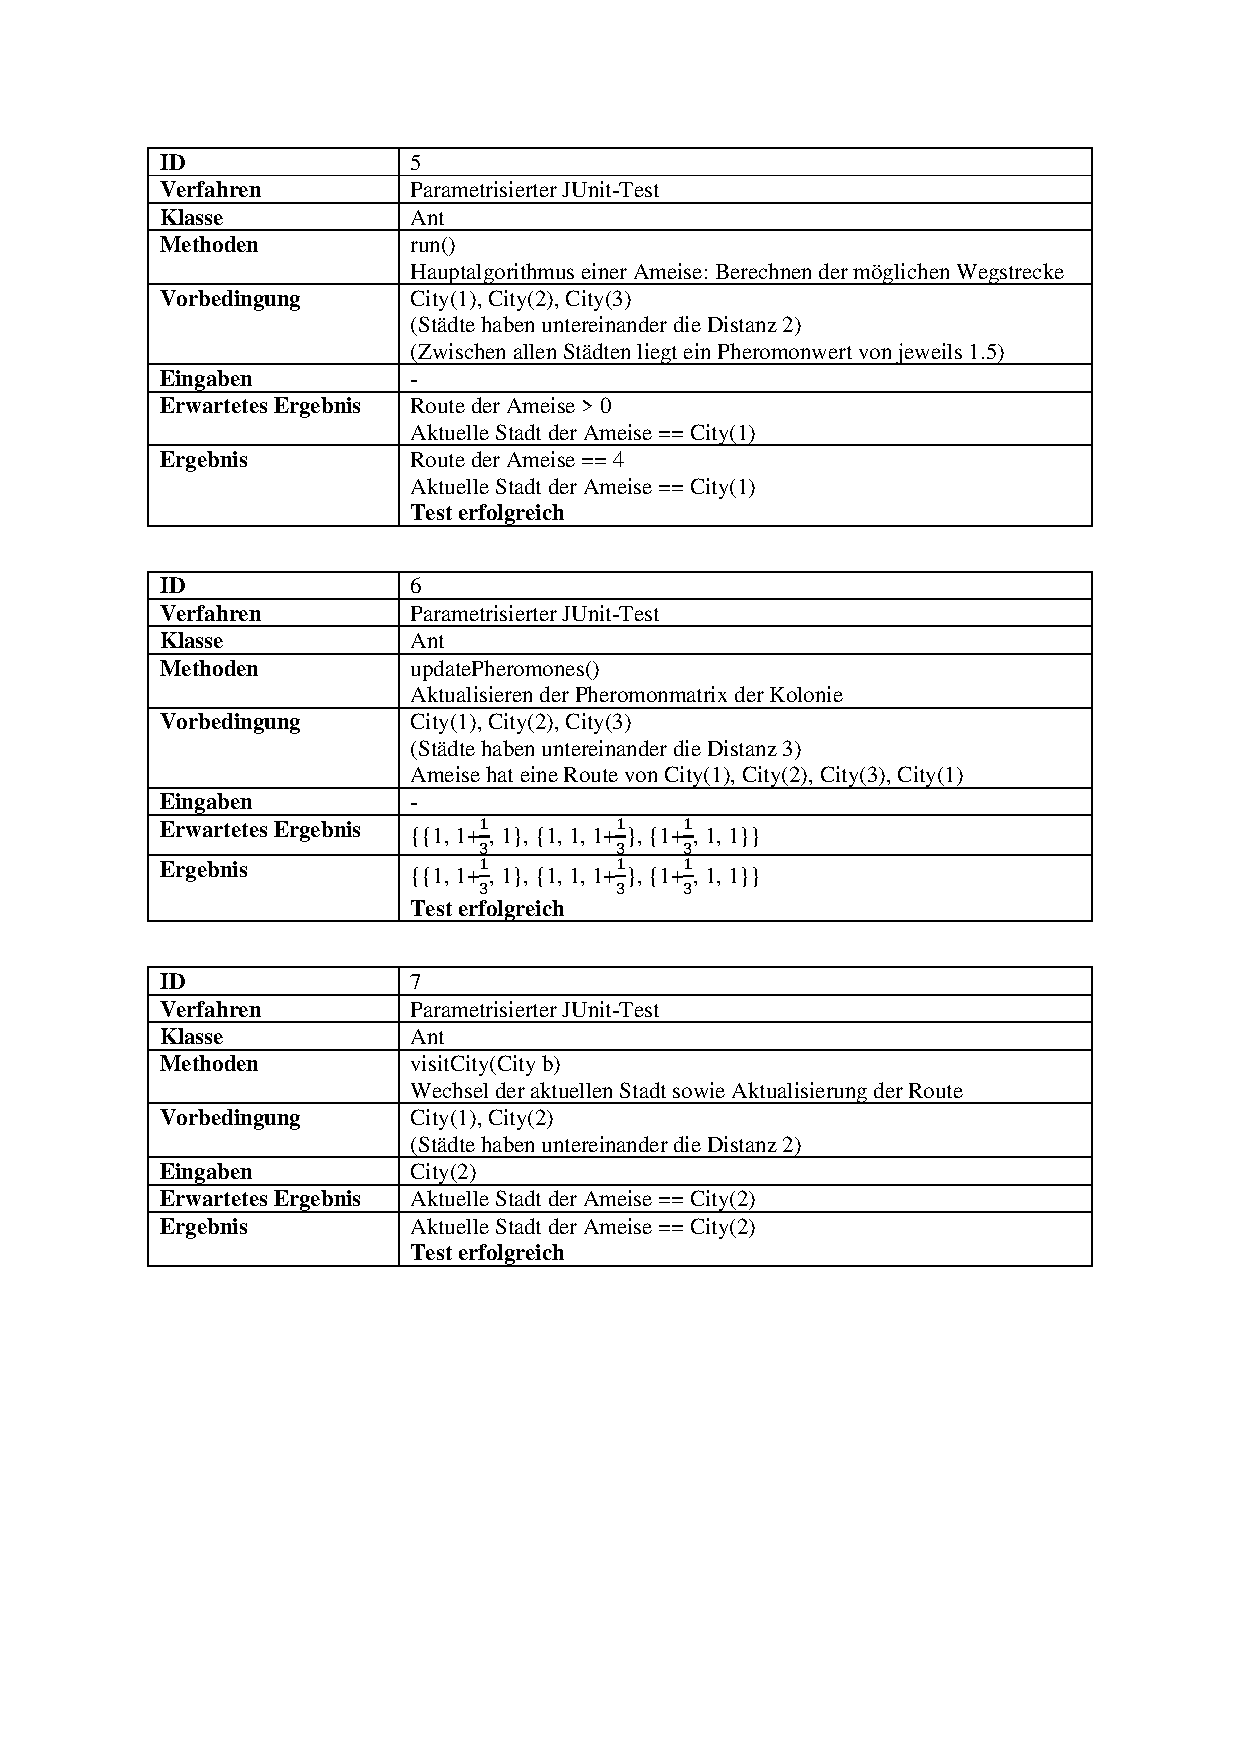
\includegraphics[width=\linewidth]{images/Testfaelle_Ant_Seite_2.pdf}
		\label{testAnt2}
	\end{figure}
	\begin{figure}[h]
		\centering
		\caption{Testfälle der Klasse $Ant$, Seite 3}
		
\includegraphics[width=\linewidth]{images/Testfaelle_Ant_Seite_3.pdf}
		\label{testAnt3}
	\end{figure}

	\begin{figure}[h]
		\centering
		\caption{Testfälle der Klasse $Colony$, Seite 1}
		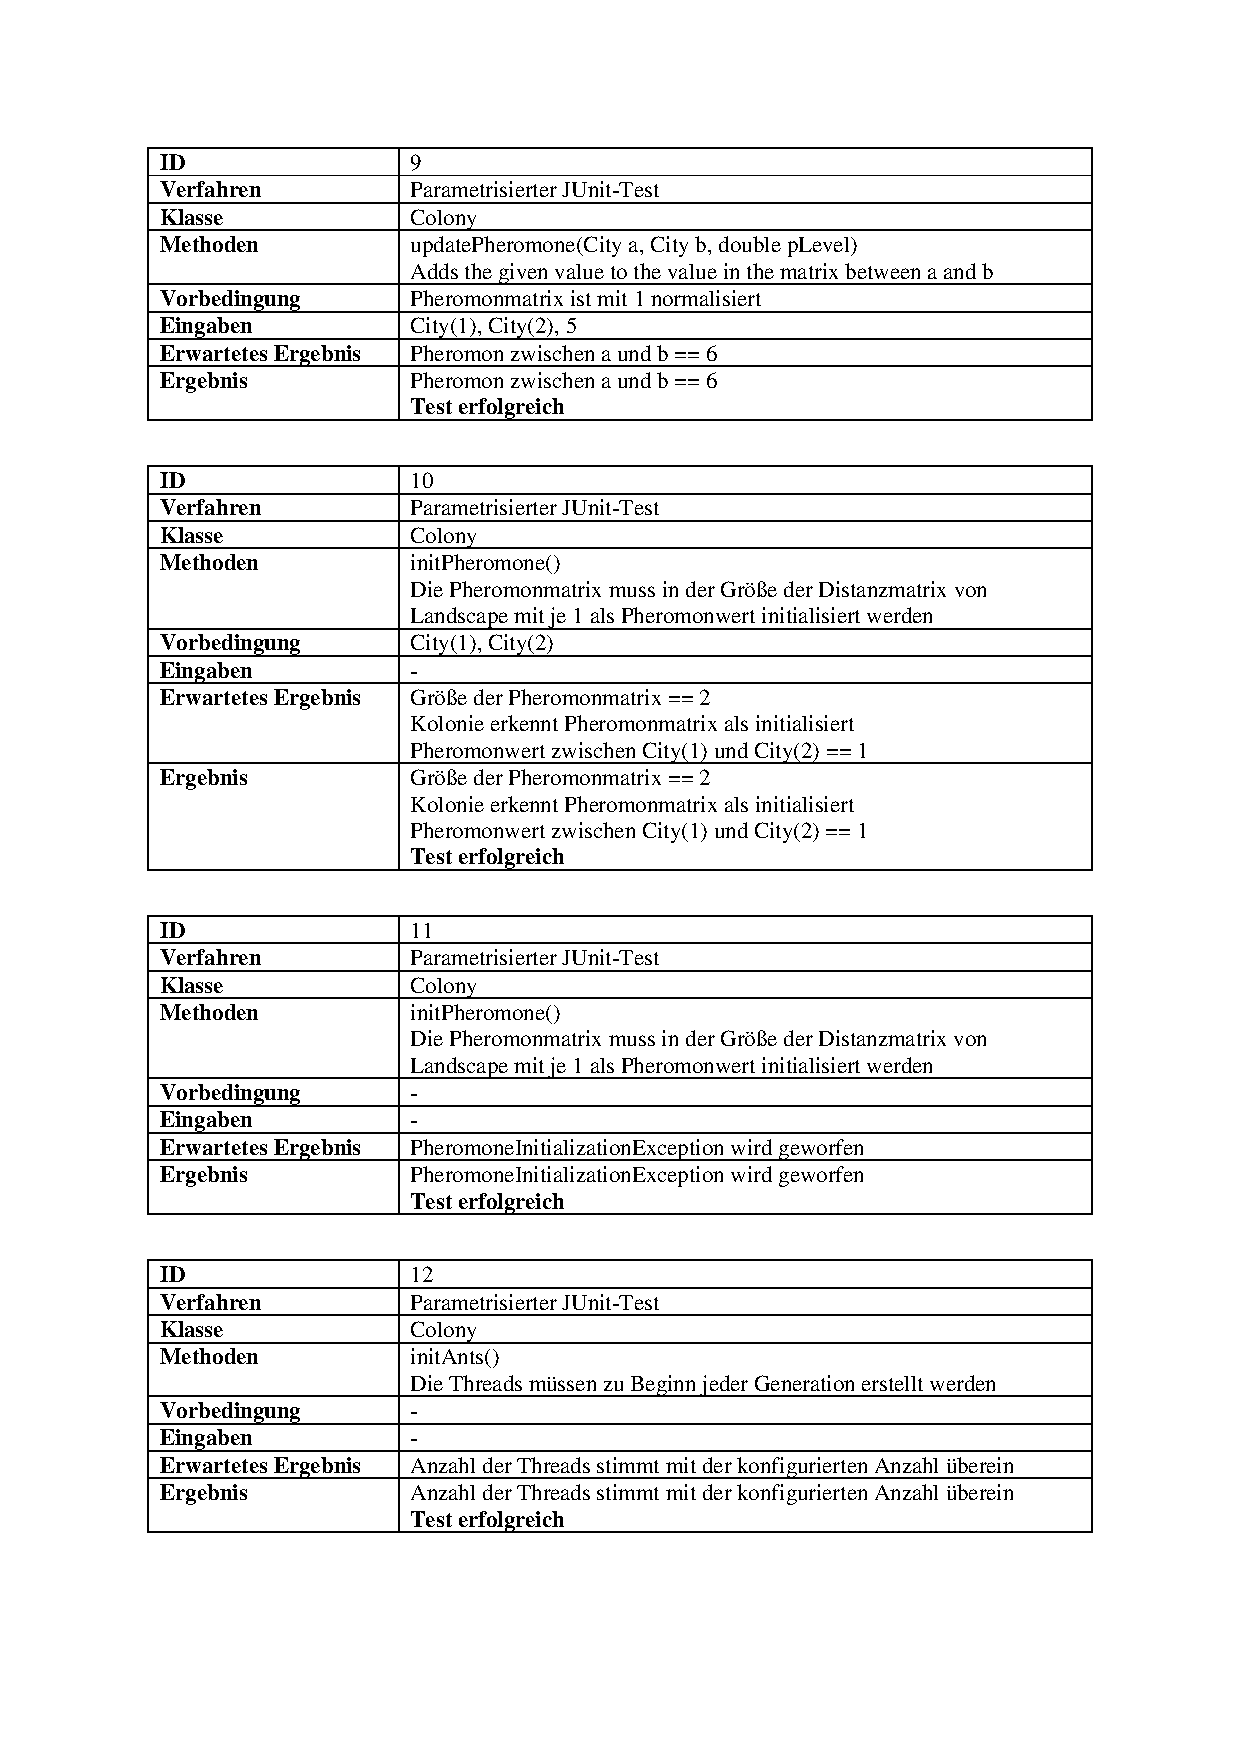
\includegraphics[width=\linewidth]{images/Testfaelle_Colony_Seite_1.pdf}
		\label{testColony1}
	\end{figure}
	\begin{figure}[h]
		\centering
		\caption{Testfälle der Klasse $Colony$, Seite 2}
		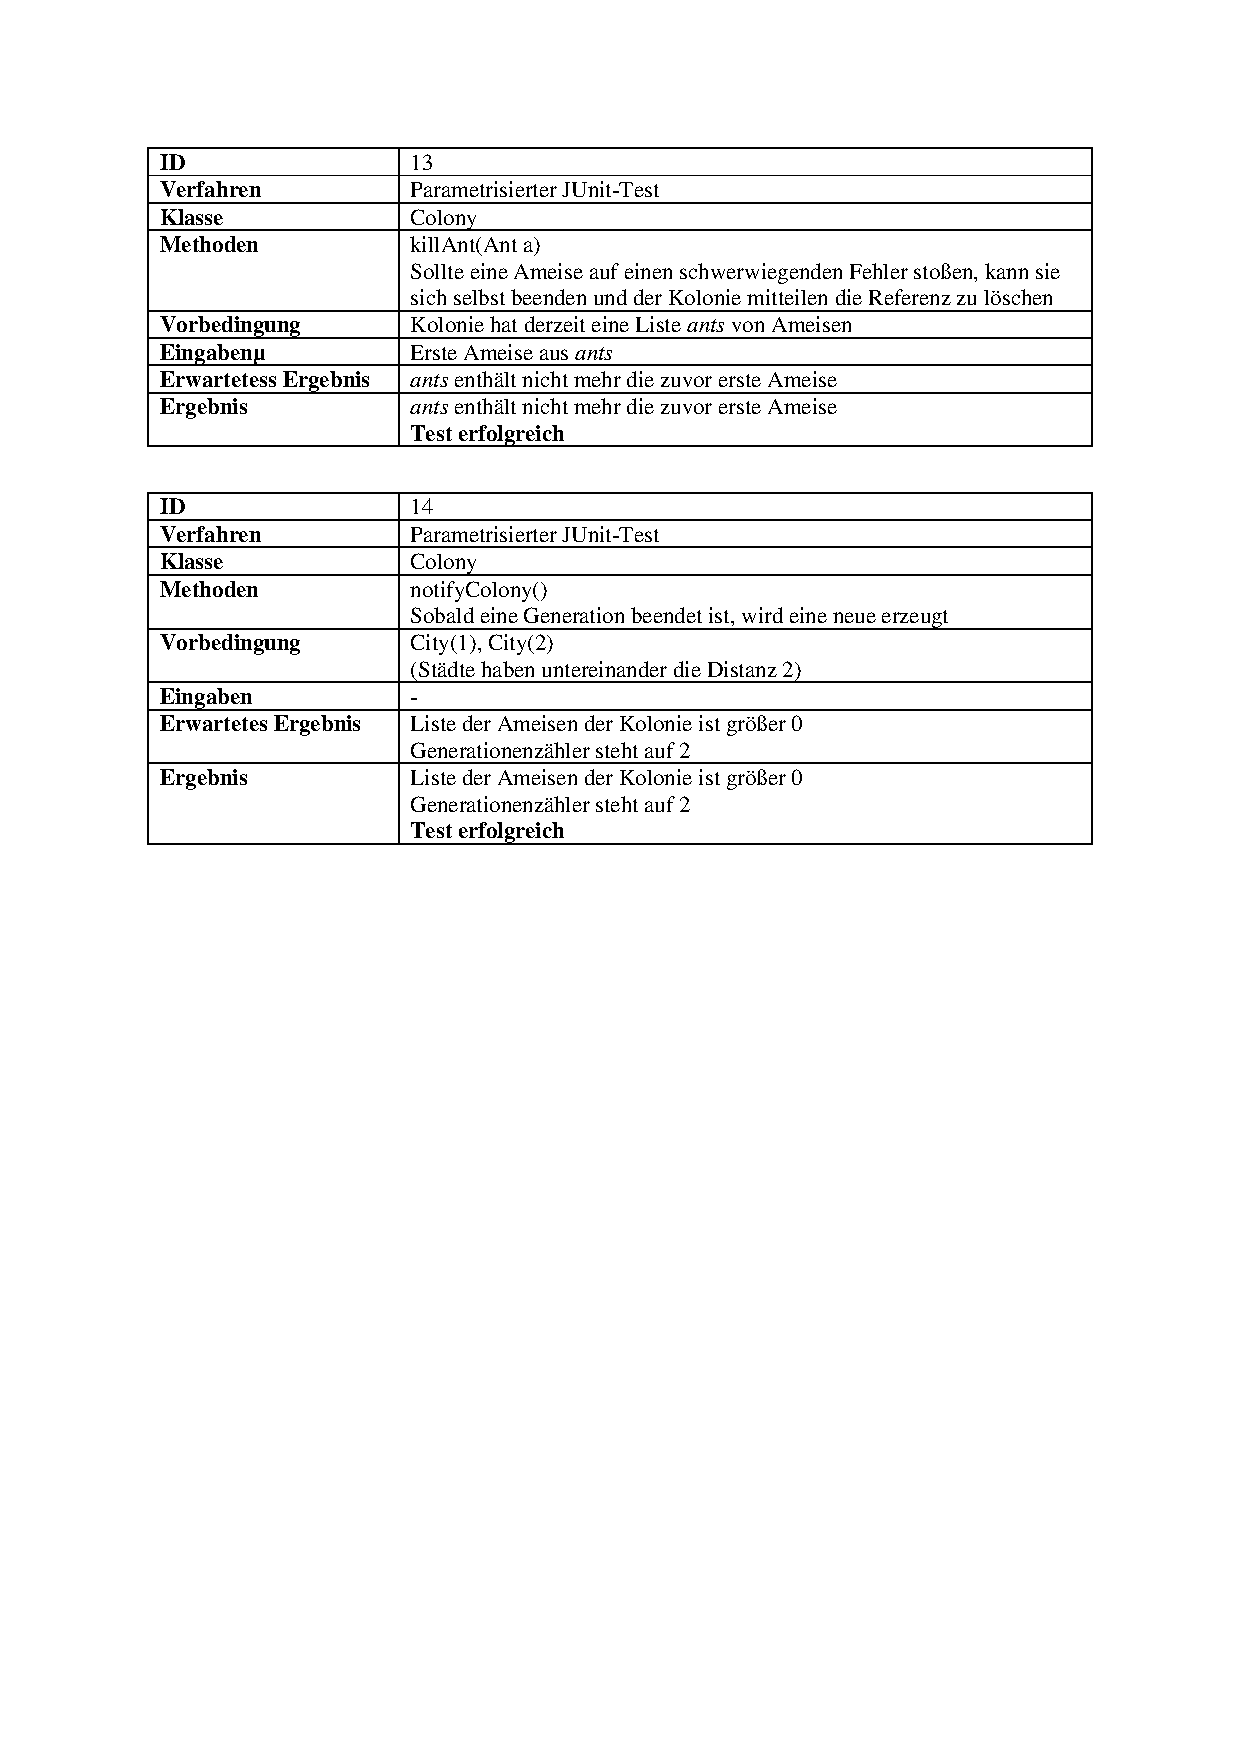
\includegraphics[width=\linewidth]{images/Testfaelle_Colony_Seite_2.pdf}
		\label{testColony2}
	\end{figure}

	\begin{figure}[h]
		\centering
		\caption{Testfälle der Klasse $Landscape$, Seite 1}
		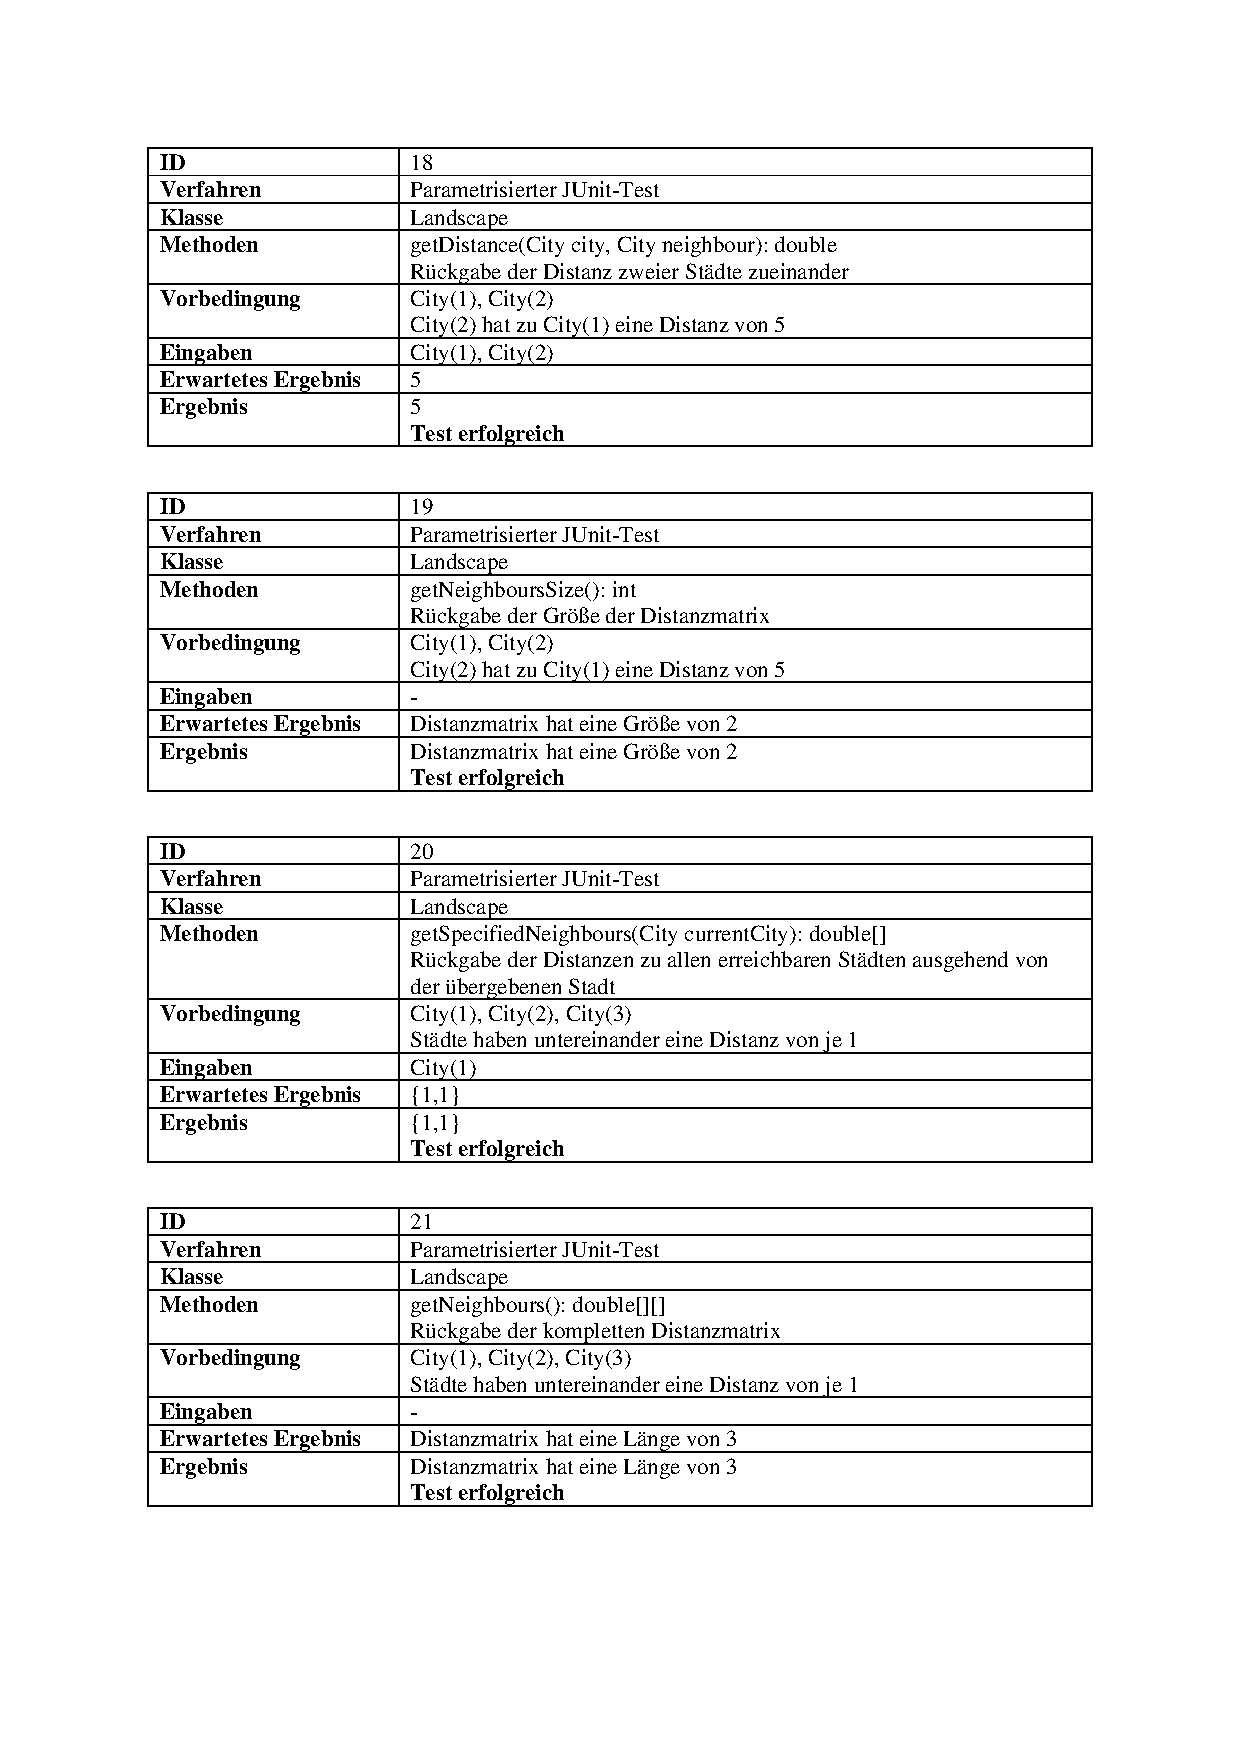
\includegraphics[width=\linewidth]{images/Testfaelle_Landscape_Seite_1.pdf}
		\label{testLandscape1}
	\end{figure}
	\begin{figure}[h]
		\centering
		\caption{Testfälle der Klasse $Landscape$, Seite 2}
		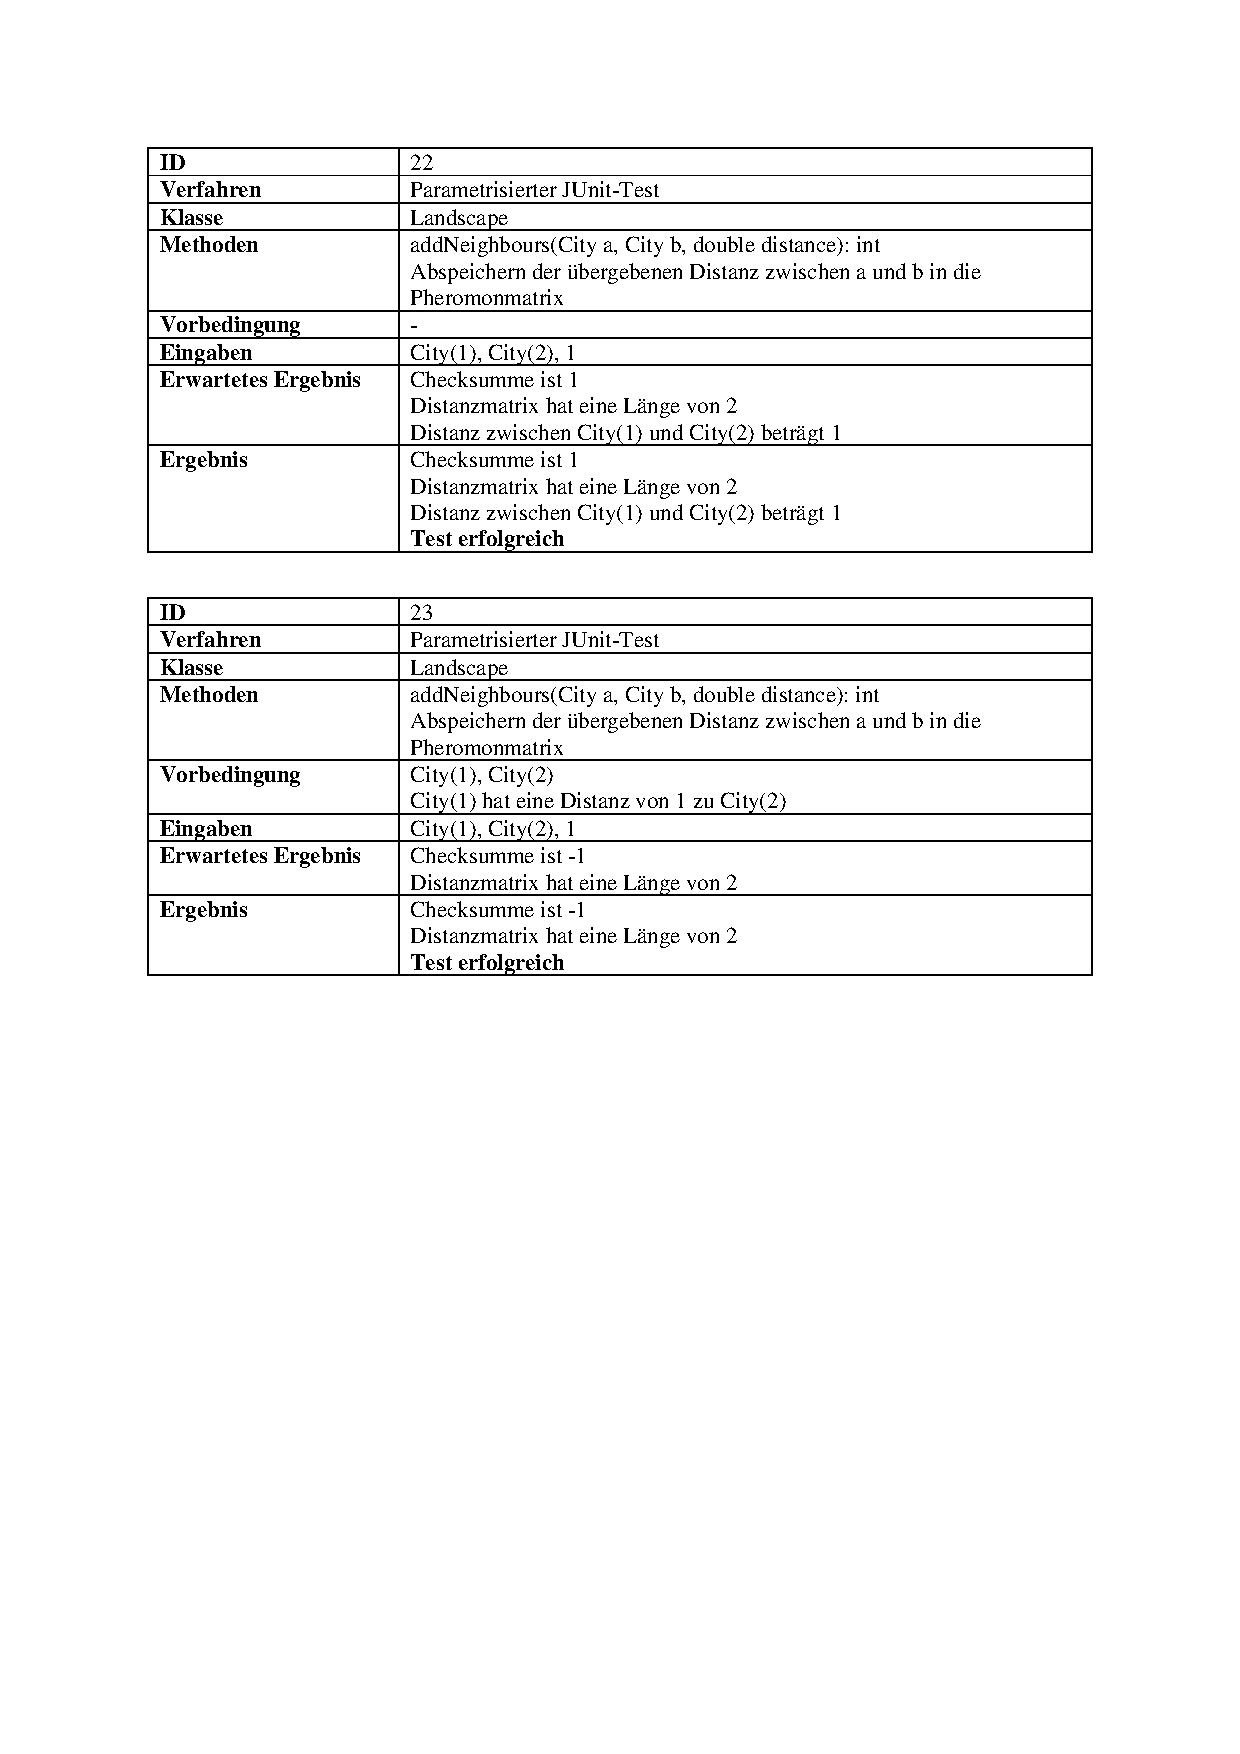
\includegraphics[width=\linewidth]{images/Testfaelle_Landscape_Seite_2.pdf}
		\label{testLandscape2}
	\end{figure}

	\begin{figure}[h]
		\centering
		\caption{Testfälle der Klassen von $Parser$}
		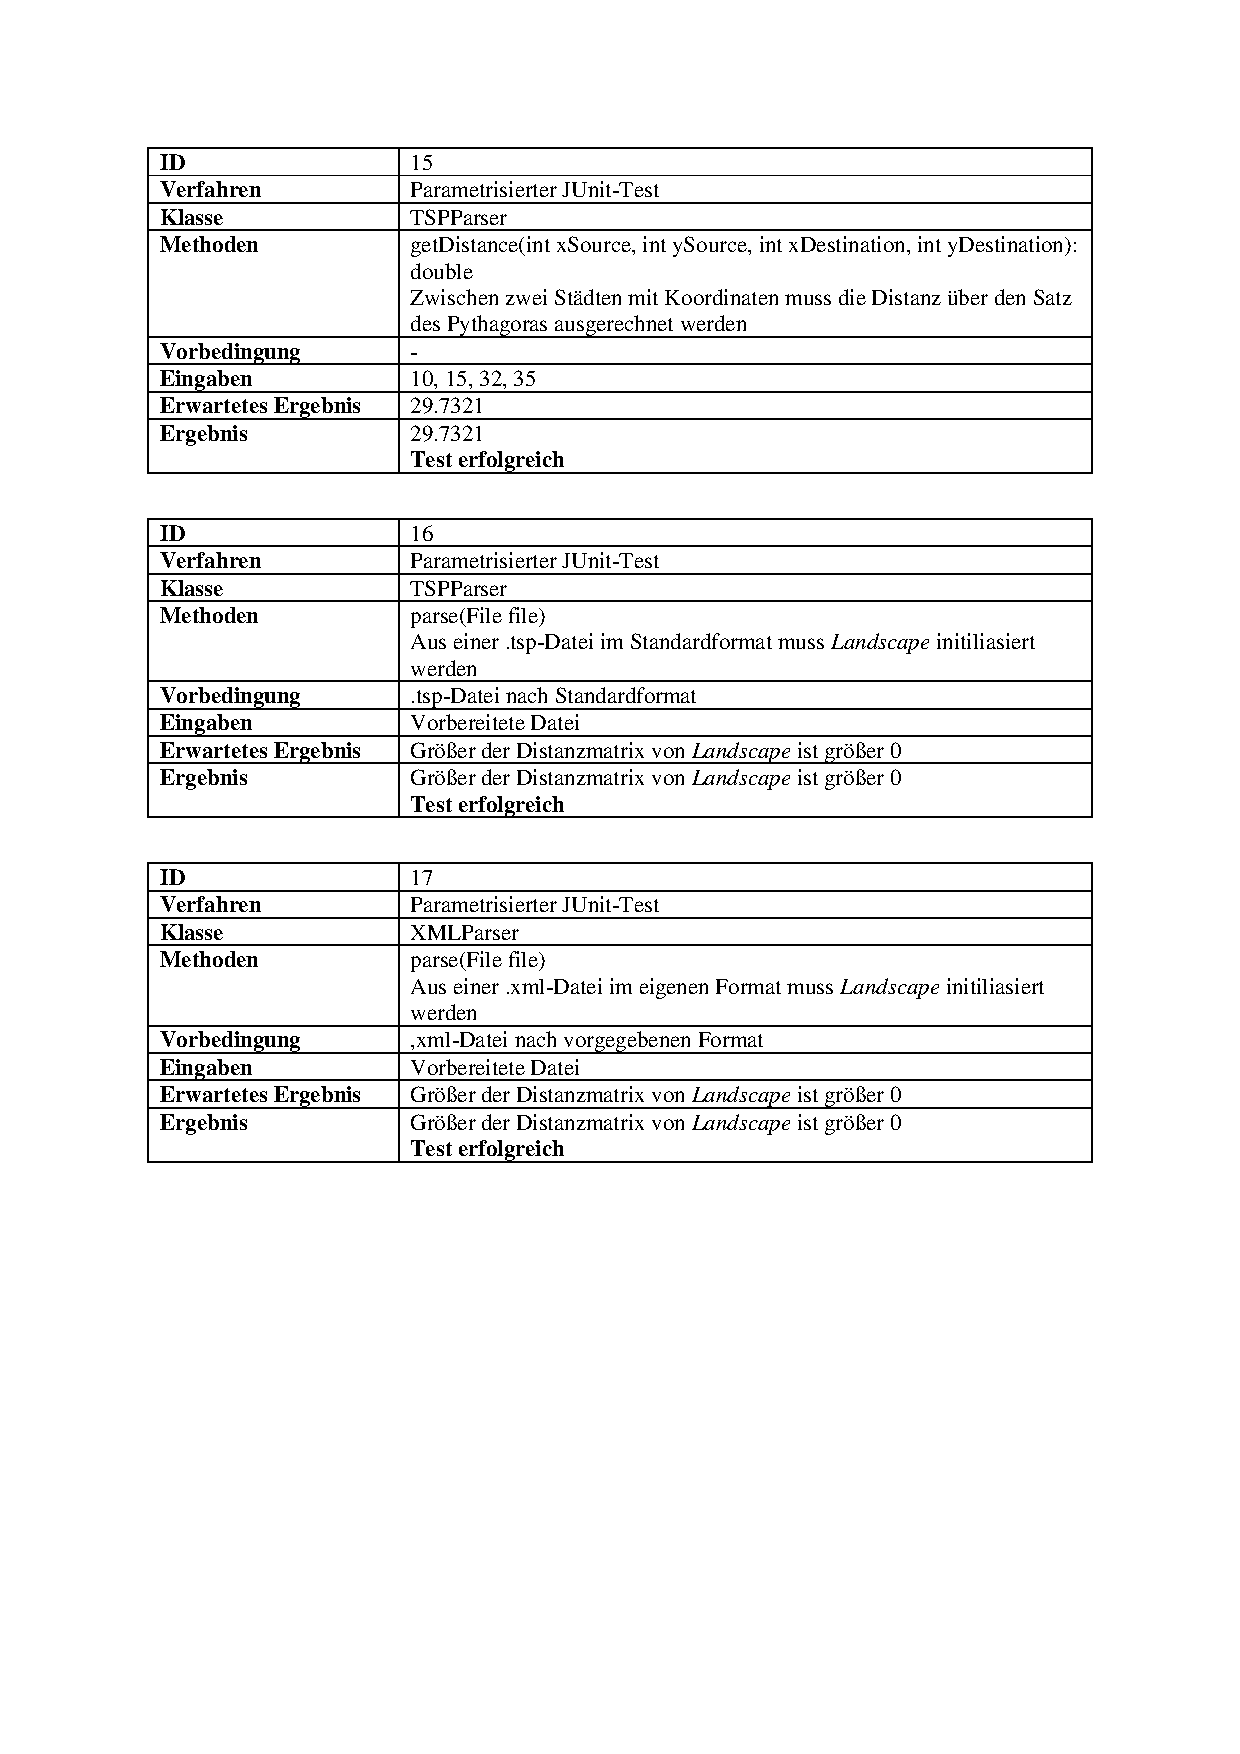
\includegraphics[width=\linewidth]{images/Testfaelle_Parser_Seite_1.pdf}
		\label{testParser1}
	\end{figure}

	\begin{figure}[h]
		\centering
		\caption{Testfälle der Klasse $HSQLDBManager$, Seite 1}
		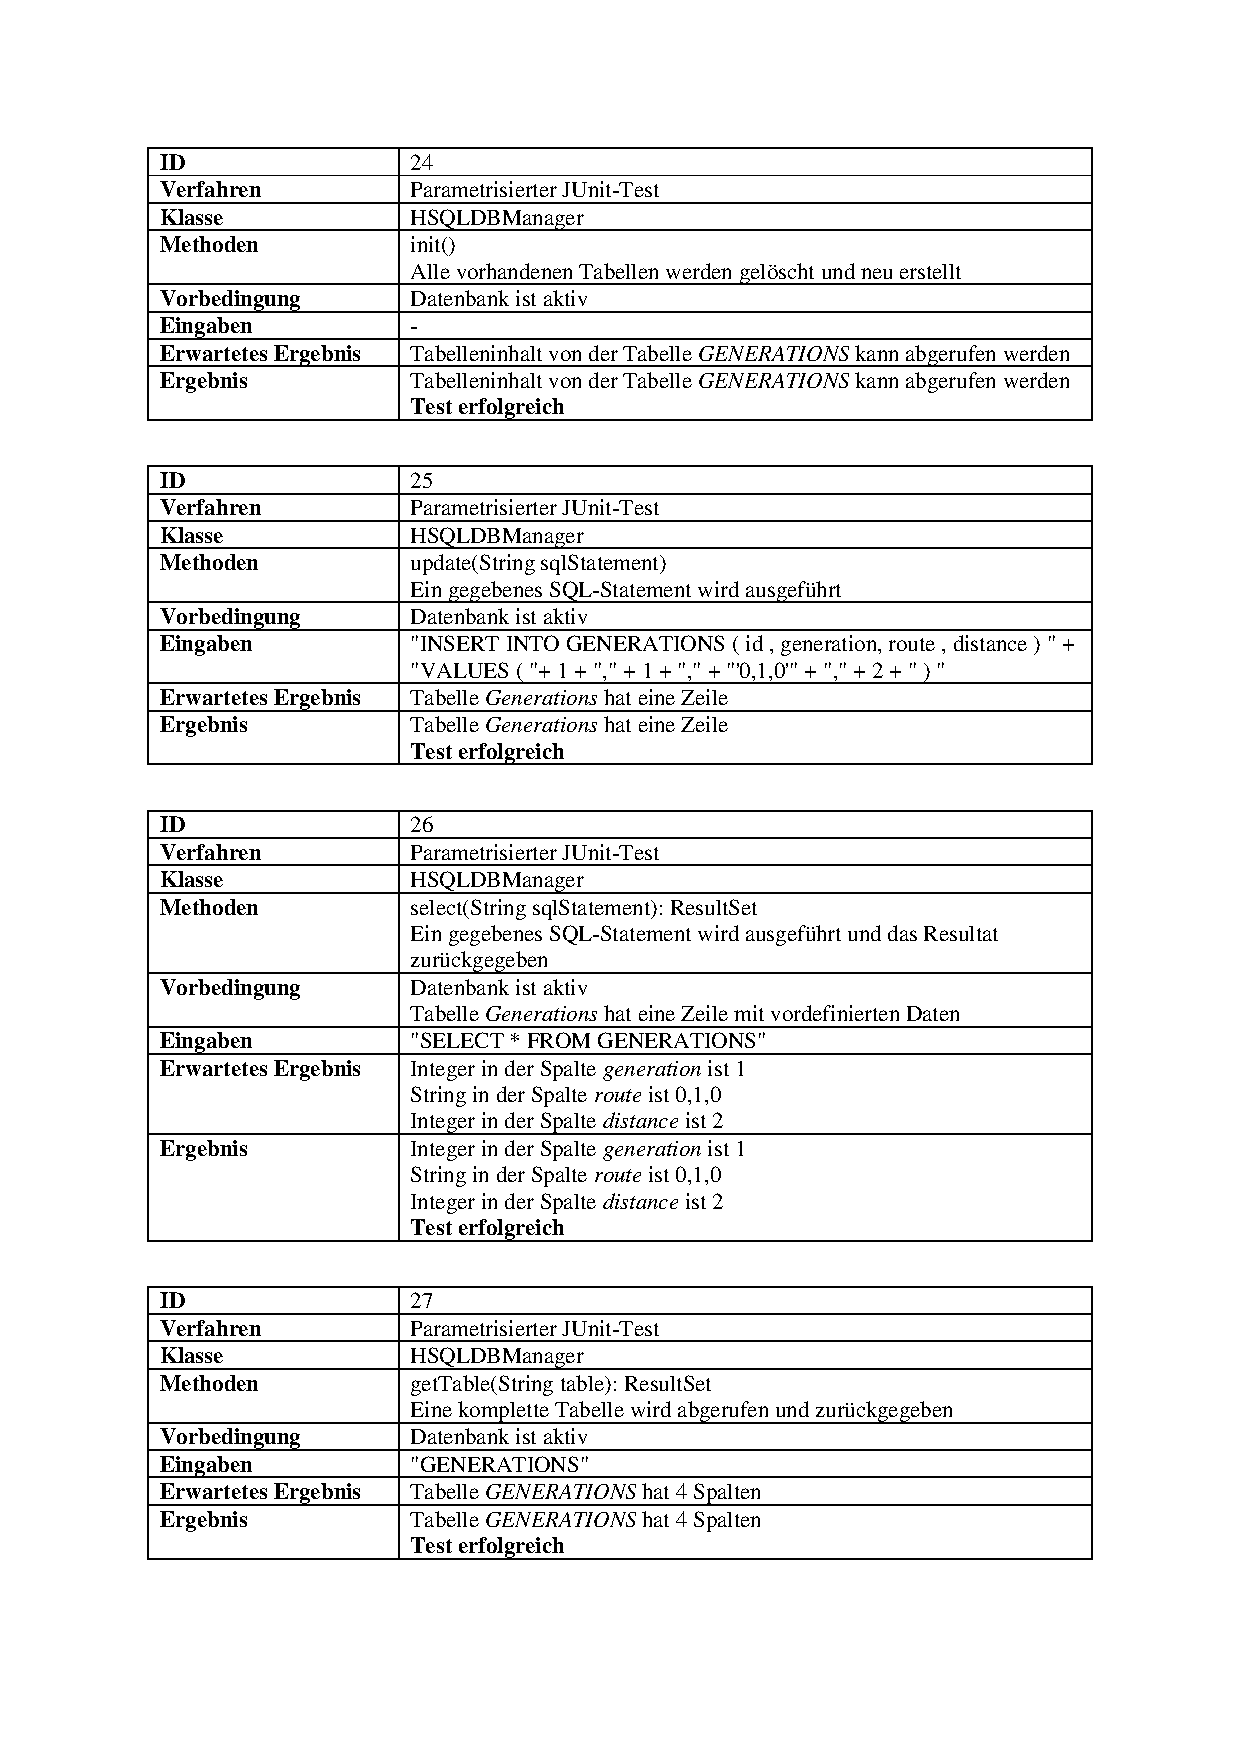
\includegraphics[width=\linewidth]{images/Testfaelle_HSQLDB_Seite_1.pdf}
		\label{testHSQLDB1}
	\end{figure}
	\begin{figure}[h]
		\centering
		\caption{Testfälle der Klasse $HSQLDBManager$, Seite 2}
		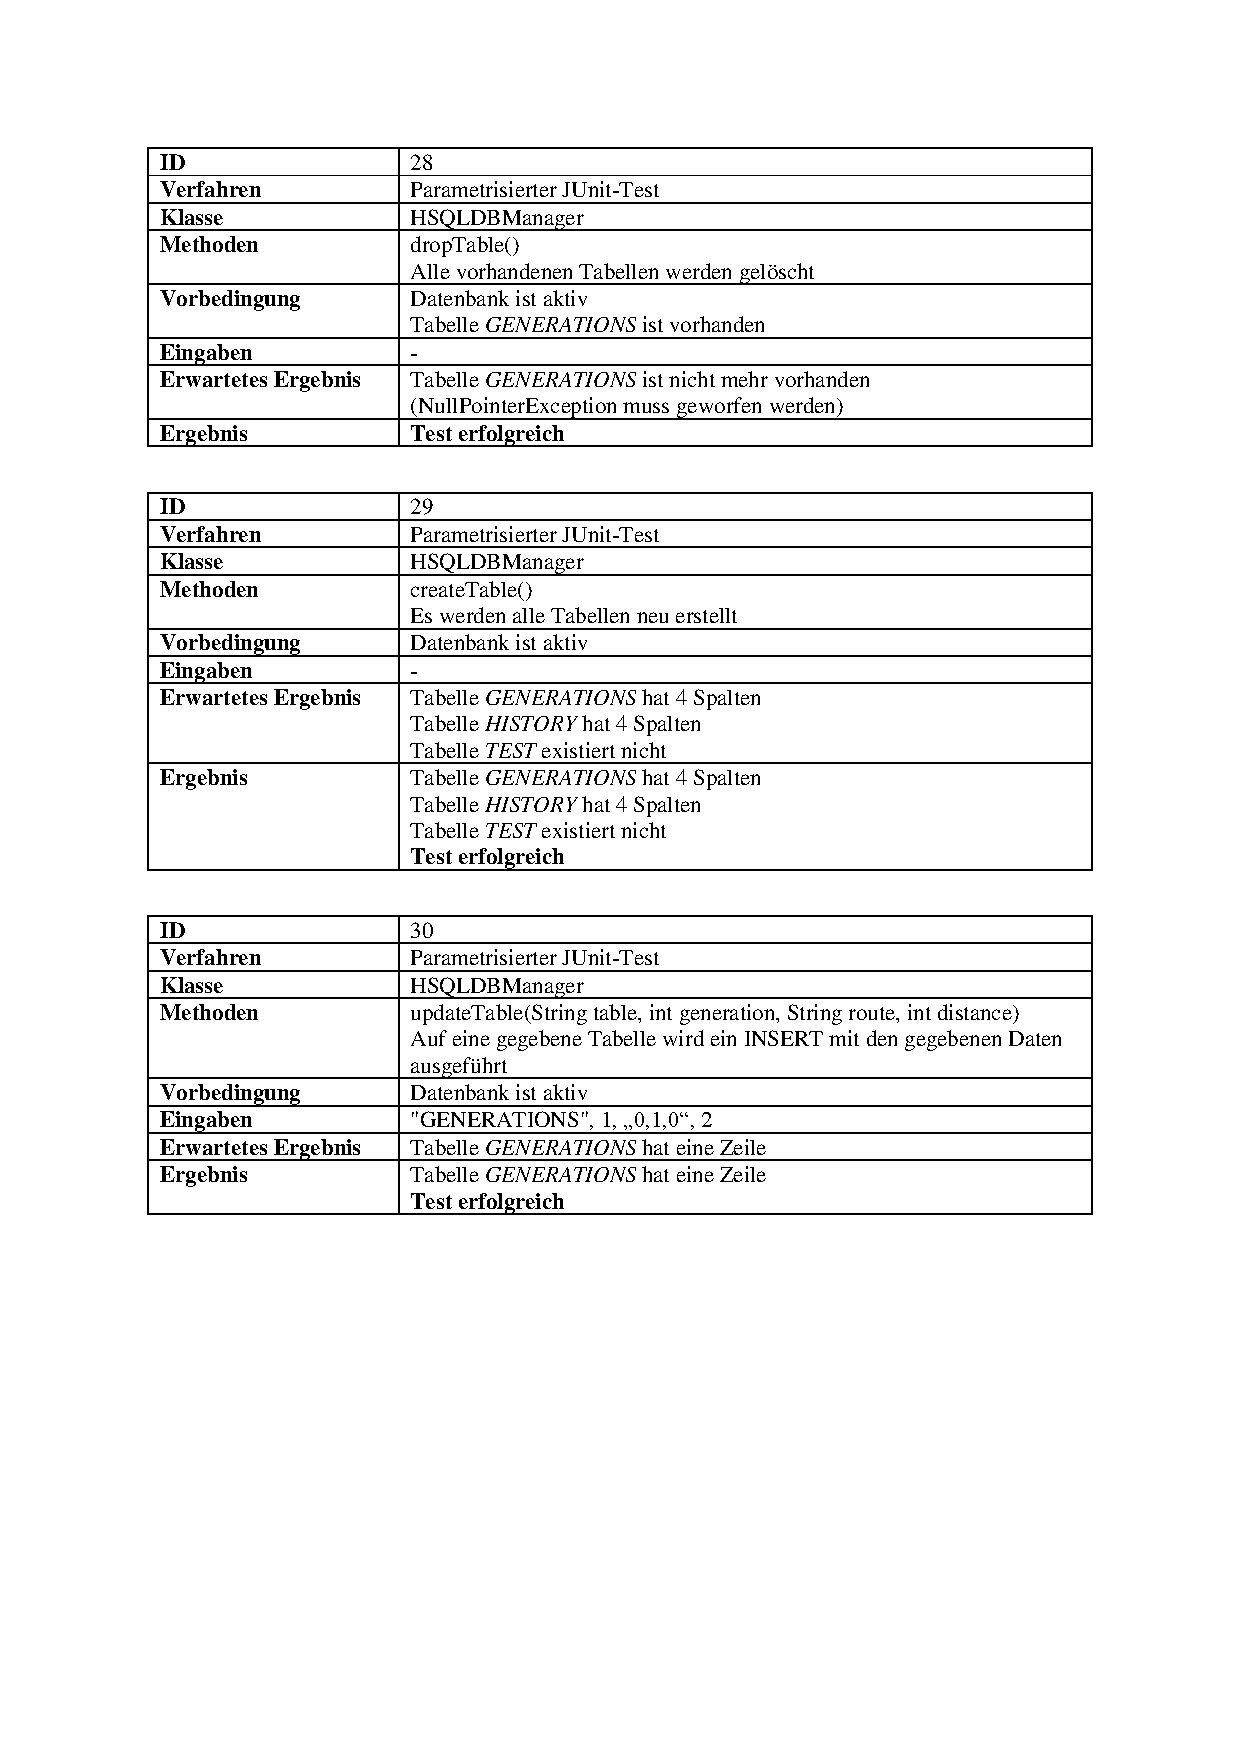
\includegraphics[width=\linewidth]{images/Testfaelle_HSQLDB_Seite_2.pdf}
		\label{testHSQLDB2}
	\end{figure}
\end{appendices}